\section{Risultati}\label{sec:risultati}
Le analisi statistiche restituiscono un quadro inequivocabile: esiste una discrepanza sistematica e gravissima tra le due fonti di dati.

\begin{figure}[H]
    \centering
    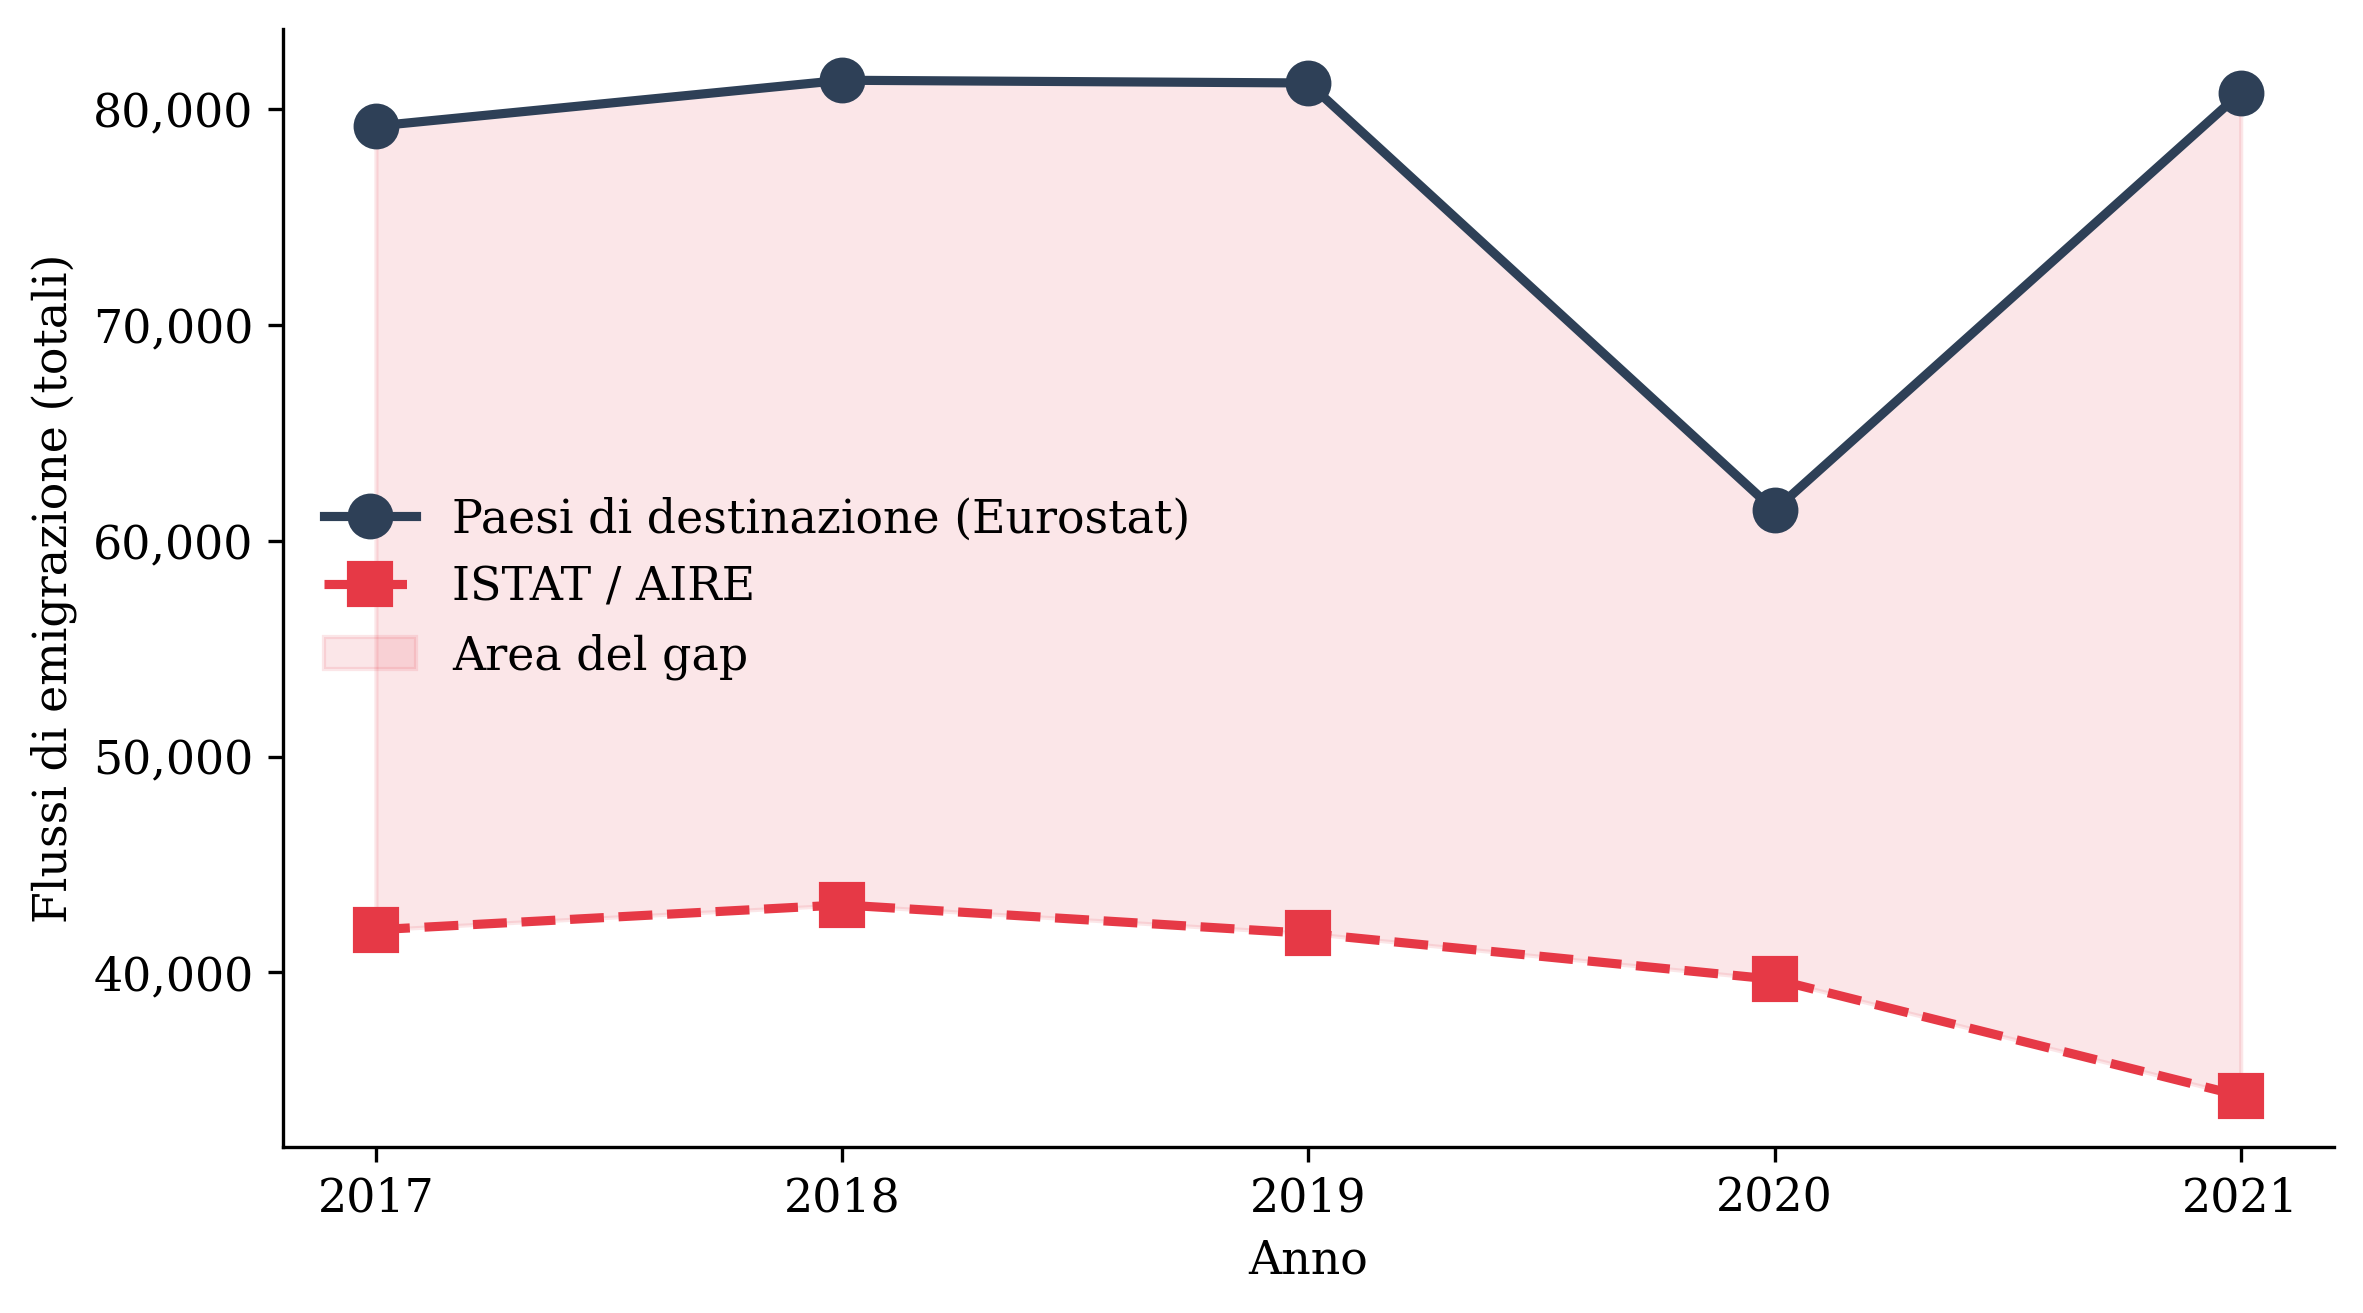
\includegraphics[width=\linewidth]{scripts/figures/fig1_trend}
    \caption{Trend dei flussi migratori aggregati (2017-2021): l'area ombreggiata quantifica l'immenso divario tra le registrazioni Eurostat (superiori) e le cancellazioni ISTAT.}
    \label{fig:trend}
\end{figure}

\subsection{Sottoconteggio Assoluto: Test di Wilcoxon}
I risultati del Wilcoxon Signed-Rank test smontano completamente l'ipotesi di errori casuali di rilevazione.
Sul dataset globale ($N=40$), il test ha generato una statistica $W = 34.0$ con un p-value microscopico di $4.3 \times 10^{-7}$.
In un campione di queste dimensioni, l'assenza di bias avrebbe prodotto un $W \approx 410$; il valore di 34.0 indica che quasi tutte le misurazioni Eurostat sono sistematicamente e pesantemente superiori a quelle ISTAT.
Il \textbf{gap mediano globale} per singola combinazione (paese/anno) si attesta a \textbf{918.5} unità mancanti.

Aggregando i dati sull'intero quinquennio per ogni nazione (Test Per-Country, $N=8$), la statistica $W$ è crollata a \textbf{0.0} (p-value = 0.0078).
Un valore di $W=0.0$ rappresenta la prova statistica estrema: in tutti gli 8 paesi esaminati, senza una singola eccezione, il numero cumulato di immigrati italiani dichiarati dal paese estero è sempre superiore alle cancellazioni ISTAT.
Il \textbf{gap mediano su base quinquennale} tra le due fonti per ogni paese è di \textbf{4565.5} unità fantasma.

\begin{figure}[H]
    \centering
    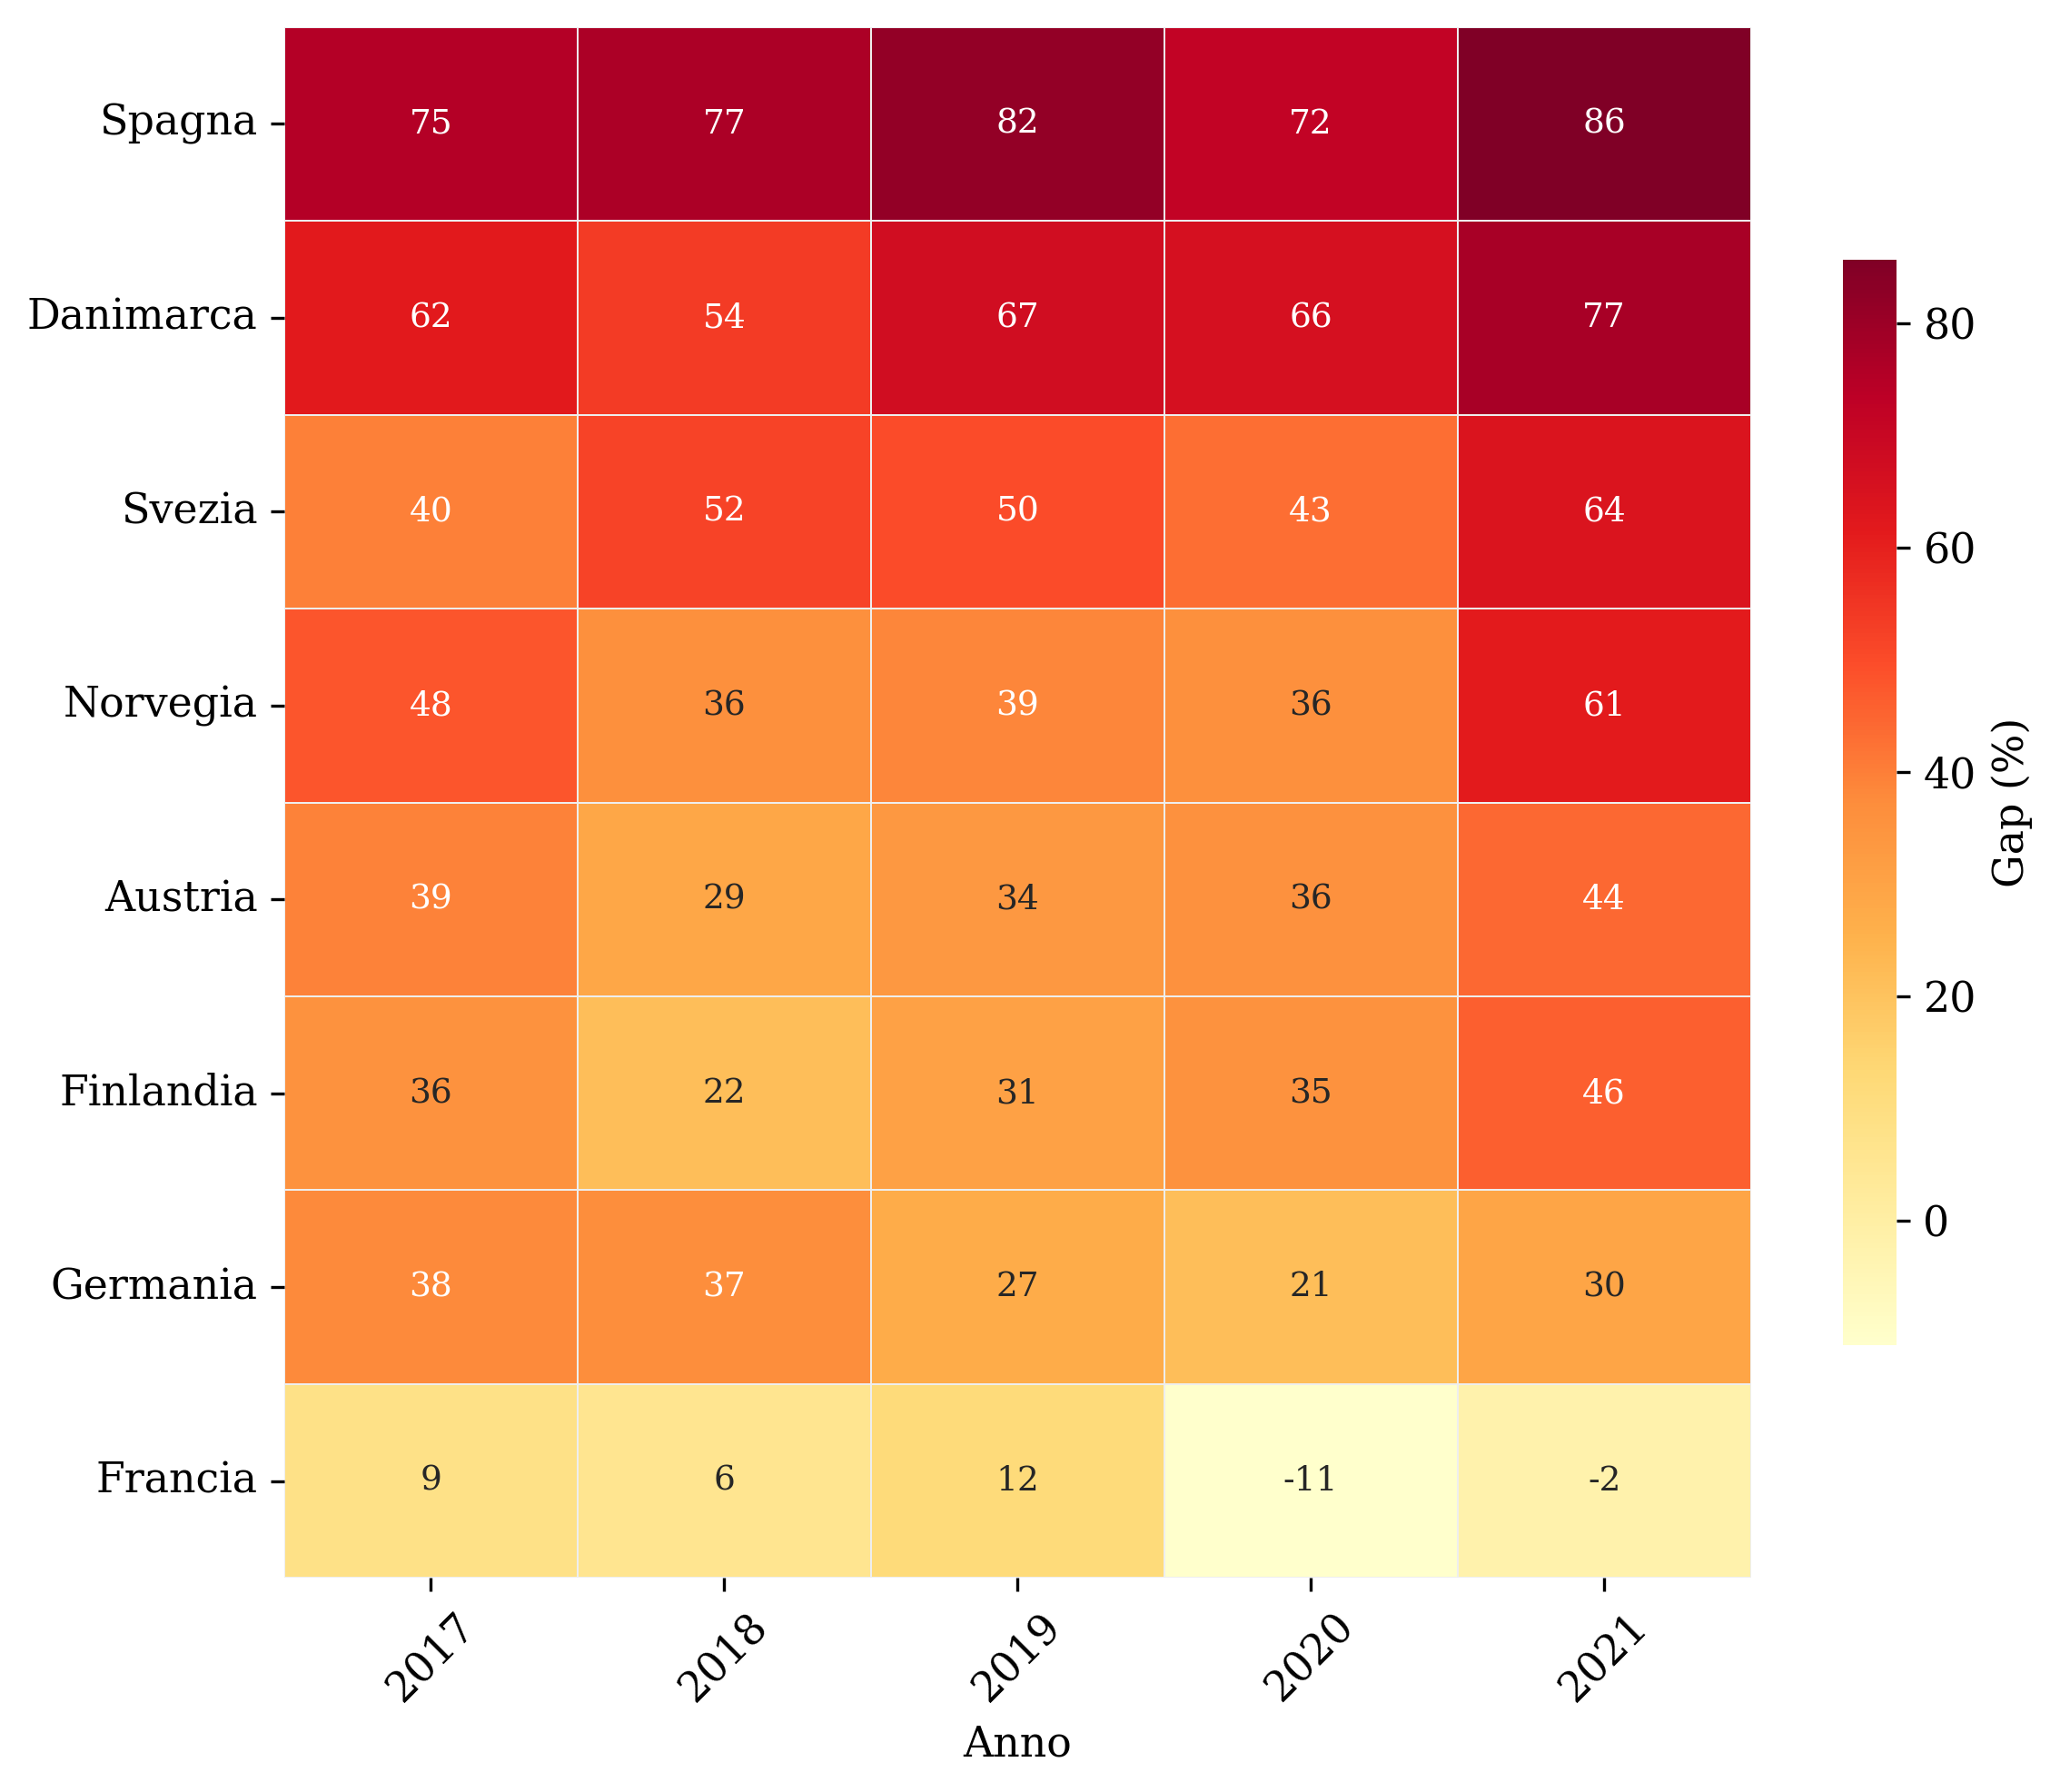
\includegraphics[width=\linewidth]{scripts/figures/fig3_heatmap}
    \caption{Heatmap del tasso di sottostima. Celle scure evidenziano percentuali critiche di mancata registrazione.}
    \label{fig:heatmap}
\end{figure}

\subsection{Sfasamento Temporale: Test del Chi-Quadrato}
L'applicazione del test del Chi-Quadrato ha dimostrato che i registri ISTAT non sono solo carenti nei volumi, ma anche scorretti nella distribuzione temporale.
Rifiutando l'ipotesi nulla per soglie di confidenza rigorose ($\alpha=0.01$), l'analisi ha registrato anomalie estreme per specifiche destinazioni.
La Spagna ($\chi^2 = 1814.088$), la Germania ($\chi^2 = 691.664$) e la Francia ($\chi^2 = 454.519$) presentano p-value di $0.000000$.
L'unica nazione con un profilo cronologico lievemente più allineato è la Finlandia ($\chi^2 = 16.758$, che non rifiuta $H_0$ a $\alpha=0.001$).
Questo significa che il ritardo burocratico della cancellazione AIRE distorce irrimediabilmente anche la comprensione di "quando" avvengono i deflussi.

\begin{figure}[H]
    \centering
    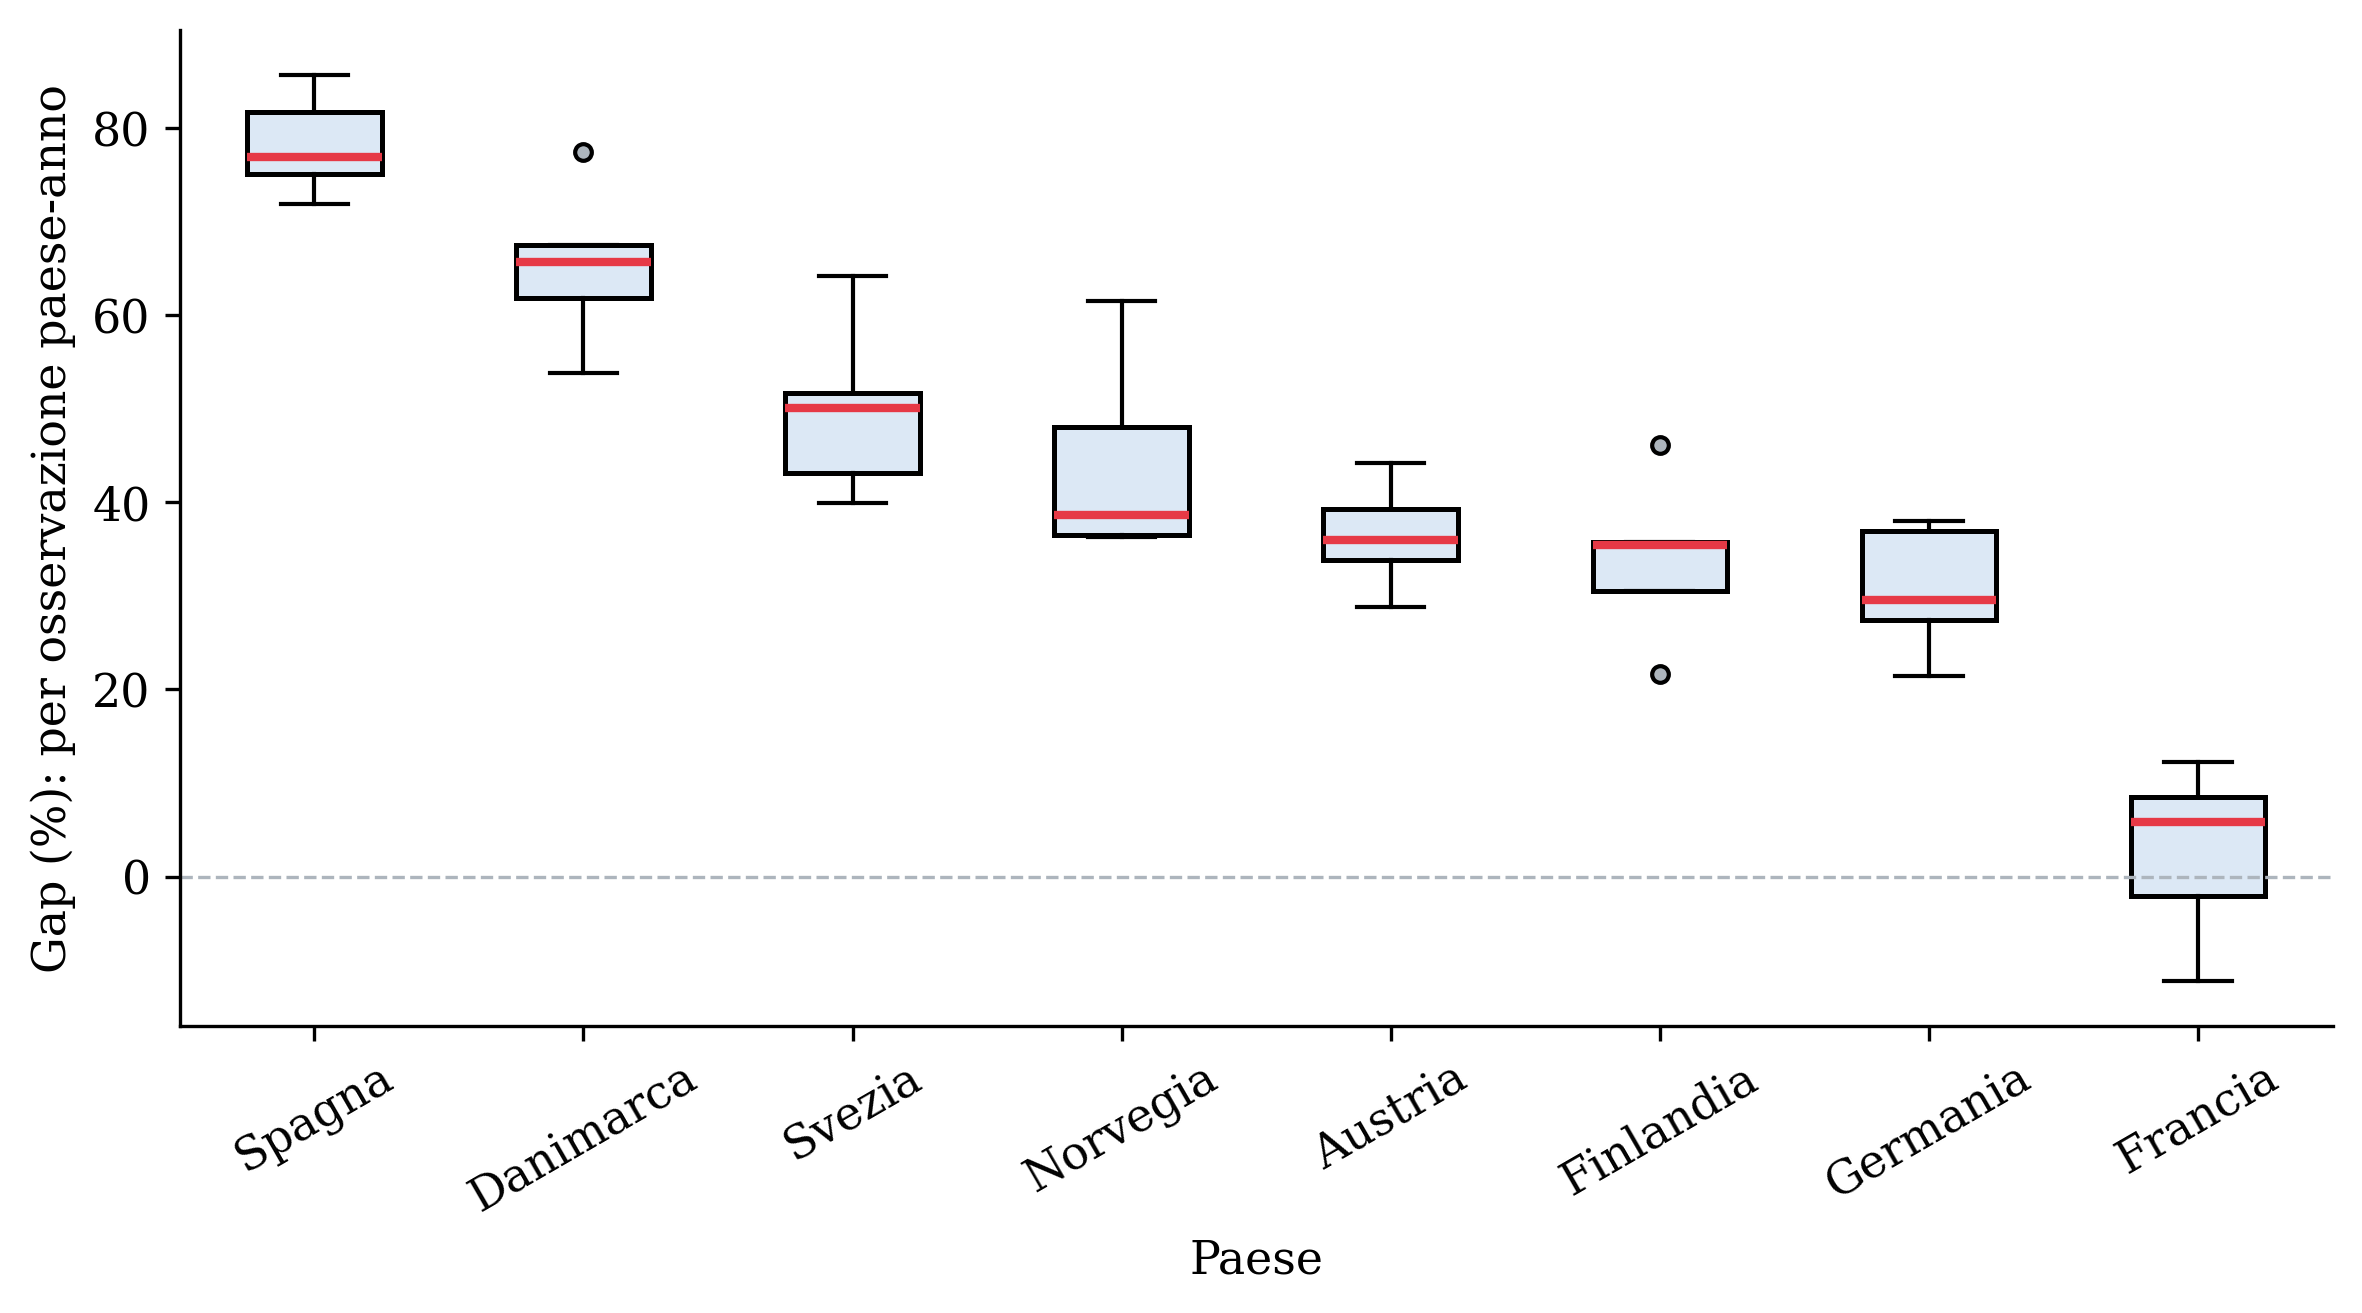
\includegraphics[width=\linewidth]{scripts/figures/fig5_boxplot}
    \caption{Boxplot della distribuzione del gap per paese: evidenzia le forti asimmetrie e l'impatto differenziale delle politiche di accoglienza locali.}
    \label{fig:boxplot}
\end{figure}